\subsection{Resultados algoritmo concurrente por hilos}

Estos fueron los tiempos de ejecución obtenidos para el algoritmo concurrente con 2 hilos:
   \begin{figure}[H]
      \centering
      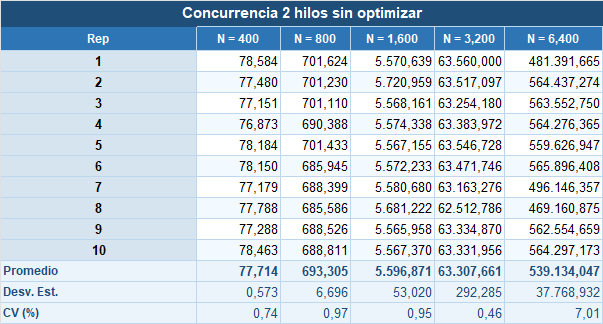
\includegraphics[width=1\textwidth]{images/tables/2threads_noopt.png}
      \caption{Tiempos de ejecución del algoritmo concurrente con 2 hilos para diferentes tamaños de matriz.}
      \label{fig:2threads}
   \end{figure}

Estos fueron los tiempos de ejecución obtenidos para el algoritmo concurrente con 4 hilos:
   \begin{figure}[H]
      \centering
      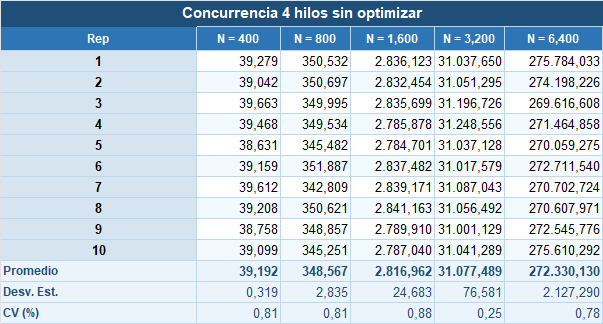
\includegraphics[width=1\textwidth]{images/tables/4threads_noopt.png}
      \caption{Tiempos de ejecución del algoritmo concurrente con 4 hilos para diferentes tamaños de matriz.}
      \label{fig:4threads}
   \end{figure}

Estos fueron los tiempos de ejecución obtenidos para el algoritmo concurrente con 6 hilos:
   \begin{figure}[H]
      \centering
      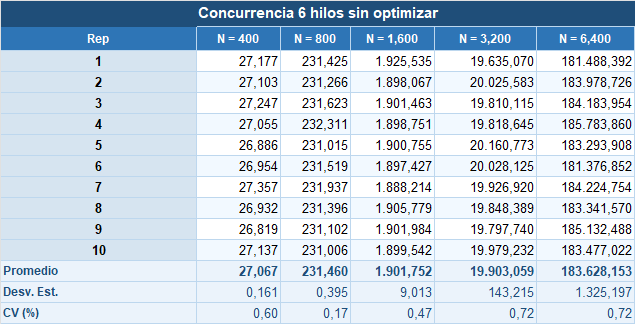
\includegraphics[width=1\textwidth]{images/tables/6threads_noopt.png}
      \caption{Tiempos de ejecución del algoritmo concurrente con 6 hilos para diferentes tamaños de matriz.}
      \label{fig:6threads}
   \end{figure}

Estos fueron los tiempos de ejecución obtenidos para el algoritmo concurrente con 8 hilos:
   \begin{figure}[H]
      \centering
      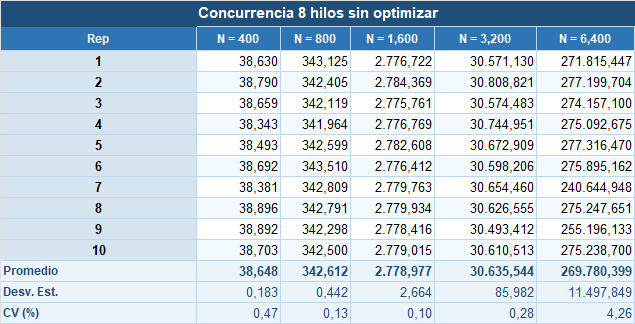
\includegraphics[width=1\textwidth]{images/tables/8threads_noopt.png}
      \caption{Tiempos de ejecución del algoritmo concurrente con 8 hilos para diferentes tamaños de matriz.}
      \label{fig:8threads}
   \end{figure}

Estos fueron los tiempos de ejecución obtenidos para el algoritmo concurrente con 12 hilos:
   \begin{figure}[H]
      \centering
      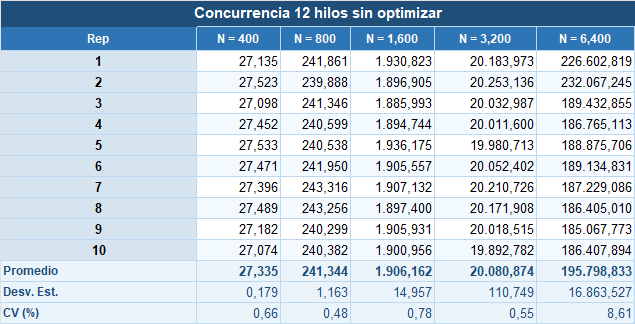
\includegraphics[width=1\textwidth]{images/tables/12threads_noopt.png}
      \caption{Tiempos de ejecución del algoritmo concurrente con 12 hilos para diferentes tamaños de matriz.}
      \label{fig:12threads}
   \end{figure}


\subsubsection{Speedup}
\label{sec:Speedup}

\begin{figure}[H]
   \centering
   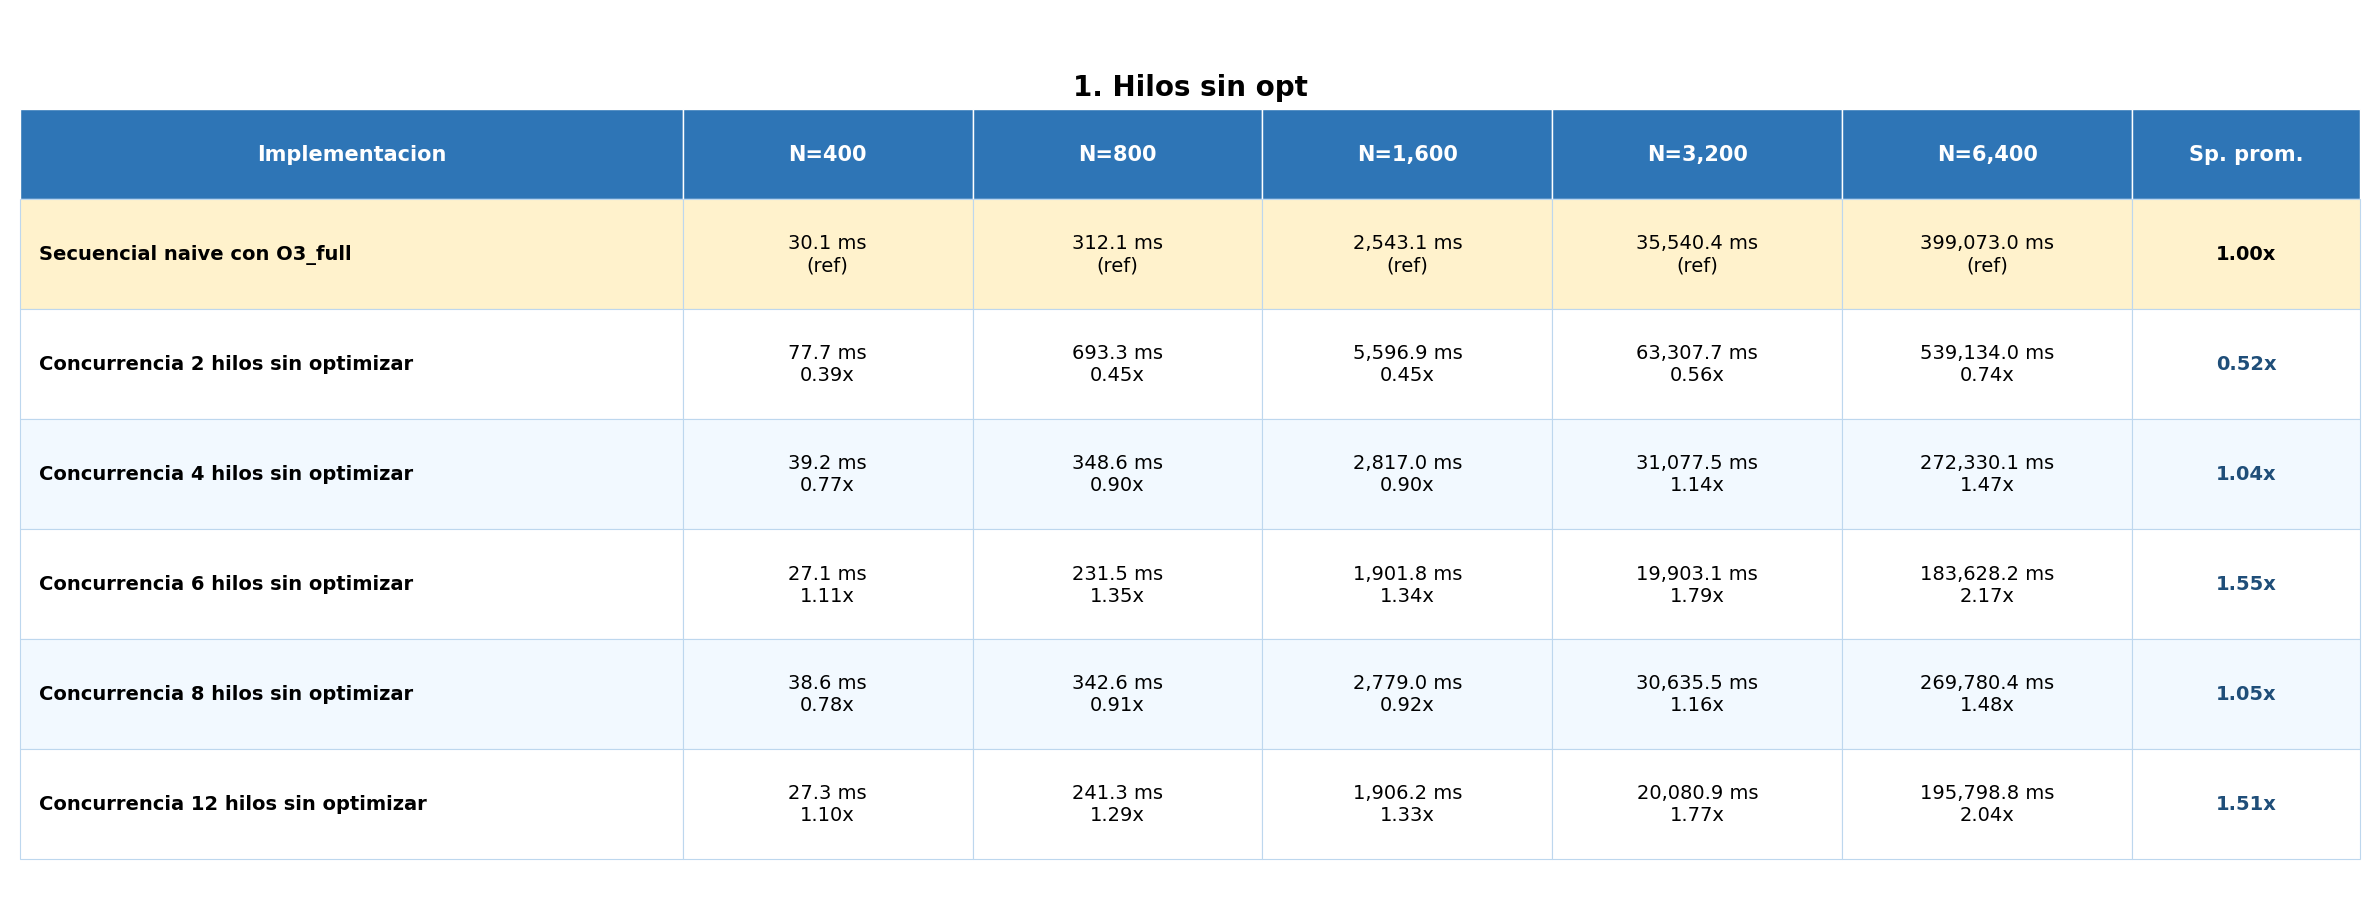
\includegraphics[width=1\textwidth]{images/tables/speedup_threads.png}
   \caption{Speedup del algoritmo concurrente con diferentes cantidades de hilos para diferentes tamaños de matriz.}
   \label{fig:speedup_threads}
\end{figure}

\begin{figure}[H]
   \centering
   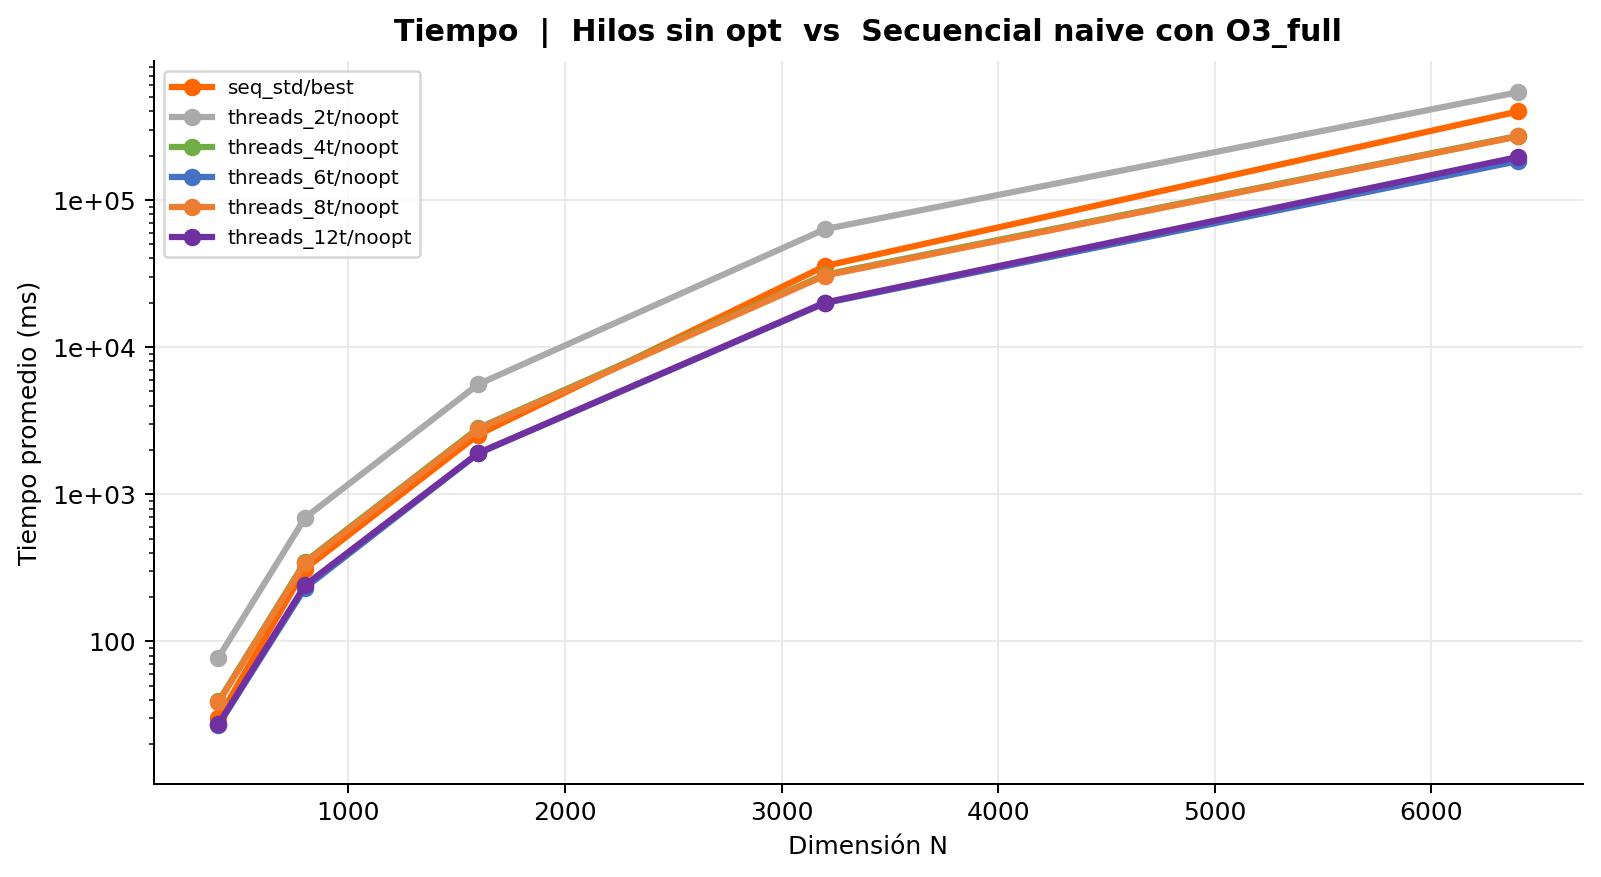
\includegraphics[width=1\textwidth]{images/charts/time_threads_noopt.png}
   \caption{Speedup del algoritmo concurrente con diferentes cantidades de hilos para diferentes tamaños de matriz (zoom).}
   \label{fig:time_threads_noopt}
\end{figure}

\begin{figure}[H]
   \centering
   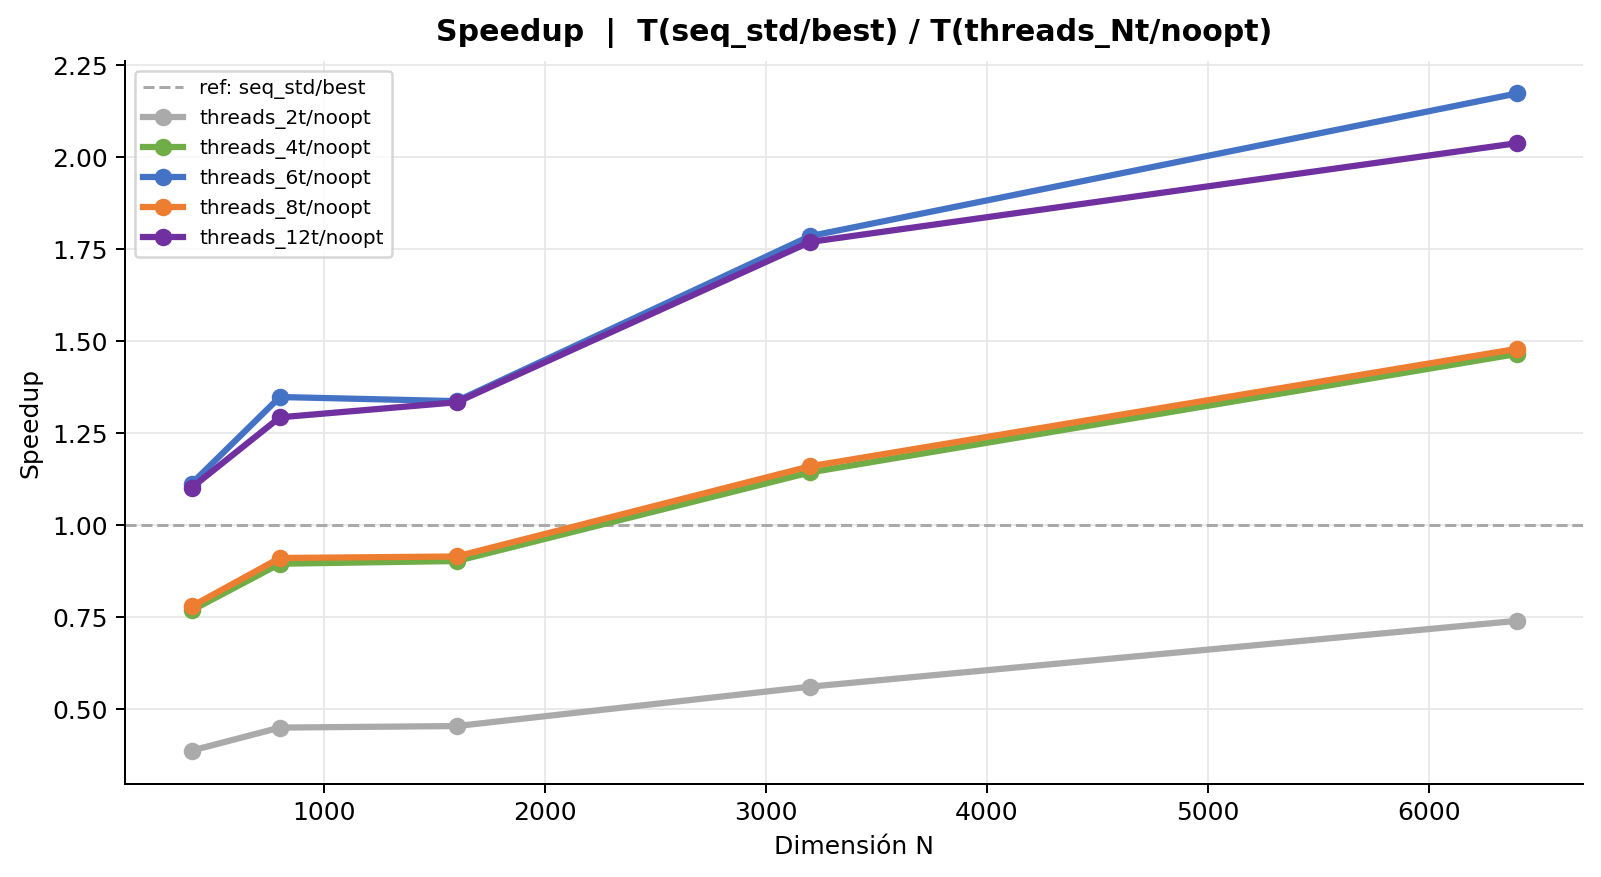
\includegraphics[width=1\textwidth]{images/charts/speedup_threads_noopt.png}
   \caption{Speedup del algoritmo concurrente con diferentes cantidades de hilos para diferentes tamaños de matriz.}
   \label{fig:speedup_threads_zoom}
\end{figure}

Como vemos en las figuras \ref{fig:speedup_threads}, \ref{fig:time_threads_noopt} y \ref{fig:speedup_threads_zoom}, el algoritmo concurrente con hilos muestra un aumento en el rendimiento a medida que se incrementa la cantidad de hilos utilizados, especialmente para matrices de mayor tamaño. Sin embargo, el Speedup no es lineal debido a factores como la sobrecarga de gestión de hilos, la contención de recursos y la eficiencia del algoritmo paralelo. En algunos casos, se observa que el rendimiento se estabiliza o incluso disminuye al agregar más hilos, lo que sugiere que existe un punto óptimo en la cantidad de hilos para cada tamaño de matriz. Si observamos el gráfico de Speedup, podemos ver que para matrices con un tamaño mayor a 3000, el rendimiento mejora significativamente con a partir de los 4 hilos, pero con solo dos hilos el rendimiento es menor. Con 12 hilos el Speedup se estabiliza o disminuye ligeramente. Esto indica que la eficiencia del algoritmo paralelo depende en gran medida del tamaño de la matriz y la cantidad de hilos utilizados, y que existe un equilibrio entre la paralelización y la sobrecarga de gestión de hilos. En este caso el que optuvo un mayor rendimiento fue utilizando 6 hilos.